\documentclass[11pt, a4paper]{article}

\usepackage[english,francais]{babel}
\usepackage[utf8]{inputenc}
\usepackage[T1]{fontenc}
\usepackage[pdftex]{graphicx}
\usepackage{setspace}
\usepackage[french]{varioref}
\usepackage{amsfonts}
\usepackage{amssymb}
\usepackage{geometry}
\usepackage{amsthm}
\usepackage[french, ruled]{algorithm2e}
\geometry{margin=2cm}

\usepackage{tikz}
\usetikzlibrary{calc}   % coordinate calculation
\usepackage{xifthen}

\title{Correctness}
\author{\'Eloi Perdereau}
%\date{}

\newcommand{\spacee}[2] {
  \begin{tikzpicture}[thick, scale=0.6]
    \def \step {1}
    \def \cc {\step/2}  % center of cell
    \coordinate (offset) at ($(\cc,\cc)$);
    \draw[step=\step] (0,0) grid ($#1$);   % draw the grid, base at #1
    % draw the neighbors
    \foreach \coord in #2 {
      \coordinate[at=\coord, name=A];
      \draw ($(A) + (offset)$) circle ({\cc*0.8});
    }
  \end{tikzpicture}
}

\theoremstyle{plain}
\newtheorem{thm}{Theorem}[section]
\newtheorem{lem}[thm]{Lemma}
\newtheorem{prop}[thm]{Proposition}
\newtheorem*{cor}{Corollary}

\theoremstyle{definition}
\newtheorem{defn}{Definition}[section]
\newtheorem{conj}{Conjecture}[section]
\newtheorem{exmp}{Example}[section]

\theoremstyle{remark}
\newtheorem*{rem}{Remark}
\newtheorem*{note}{Note}

\begin{document}

\maketitle

We define the \textit{bounding box} $BB(t)$ of the robots as the smallest
enclosing rectangle (oriented with the grid's axes) which contains all robots
at step $t$.

\begin{prop}
When following the algorithm described above, the bounding box of the robots is
monotonically non-inflating, i.e., $BB(t+1) \subseteq BB(t)$ for all $t$.
\end{prop}

\section{A single robot on the topmost row}

We note $r(t)$ the single robot in the topmost row of the bounding box at step
$t$. If there are more than one robot, $r(t)$ is not defined.

\begin{prop}
If $r(t)$ exists and is on $(0,i)$, then there is a robot on $(0,i-1)$, $(0,i)$
or $(0,i+1)$ at step $t-1$.
\end{prop}

\begin{lem}
If $r(t)$ exists and there are at least three robots in the space, then after a
constant number of steps, either $BB(t+c) \subset BB(t)$ (the topmost row moves
down) or it becomes an end case
\end{lem}

\begin{proof}

The graph of figure \ref{graph:single} is defined as follows :
\begin{itemize}
  \item Nodes : Possible cases for a single robot $(i,j)$ on the topmost row.
  \item Edge $(u,v)$ if $u$ can lead to $v$ at $t+1$ for any robot on row $i$.
\end{itemize}

We can see that there is a cycle from case $1.2.1$ (call it $a$) to $1.2.3$
(call it $b$). So theoretically the robot on the topmost row could cycle
indefinitely. We show that this is not true :

The only cases where we pass through $(a,b)$ are : \\
\spacee {(7, 5)} {{(1, 0),(3, 1),(2, 1),(3, 2)}}
\spacee {(7, 5)} {{(1, 0),(0, 0),(3, 1),(2, 1),(3, 2)}}
\spacee {(7, 5)} {{(3, 1),(2, 1),(1, 1),(3, 2)}}
\\

Reciprocally for $(b,a)$ : \\
\spacee {(7, 5)} {{(5, 1),(4, 1),(3, 1),(3, 2)}}
\spacee {(7, 5)} {{(5, 0),(4, 1),(3, 1),(3, 2)}}
\spacee {(7, 5)} {{(6, 0),(5, 0),(4, 1),(3, 1),(3, 2)}}
\\

It is obvious that whenever the robot pass through one of the edges of the
cycle at $t$, it can't pass through the other one at $t+1$.

\end{proof}

\begin{figure}
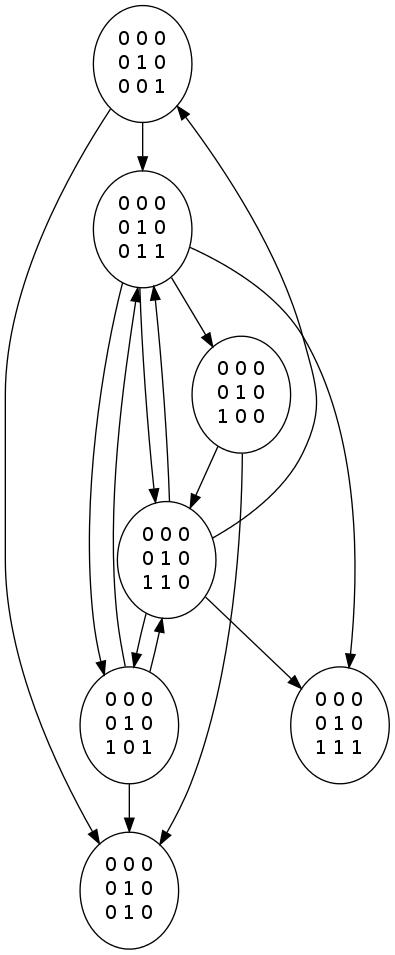
\includegraphics[scale=0.50]{graph_single_all.jpg}
\caption{Single robot}
\label{graph:single}
\end{figure}

\begin{figure}
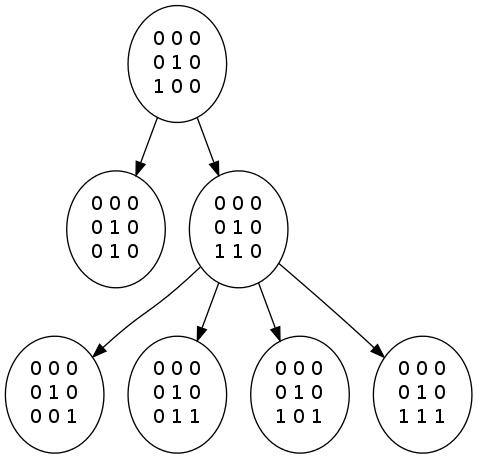
\includegraphics[scale=0.50]{graph_single_left.jpg}
\caption{Single robot go left}
\label{graph:single_left}
\end{figure}

\begin{figure}
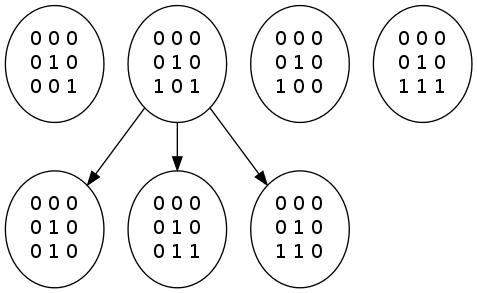
\includegraphics[scale=0.50]{graph_single_mid.jpg}
\caption{Single robot persist}
\label{graph:mid}
\end{figure}

\begin{figure}
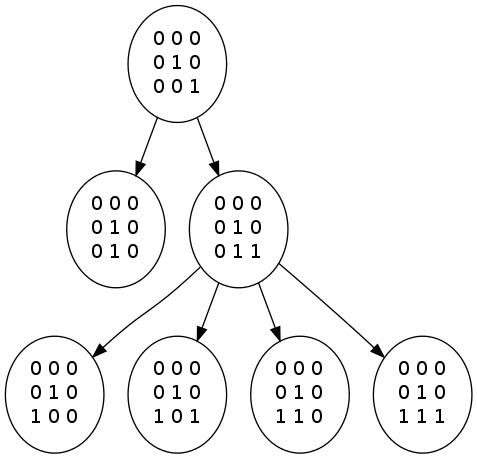
\includegraphics[scale=0.50]{graph_single_right.jpg}
\caption{Single robot go right}
\label{graph:right}
\end{figure}

\section{More than one robot on the topmost row}

\begin{figure}
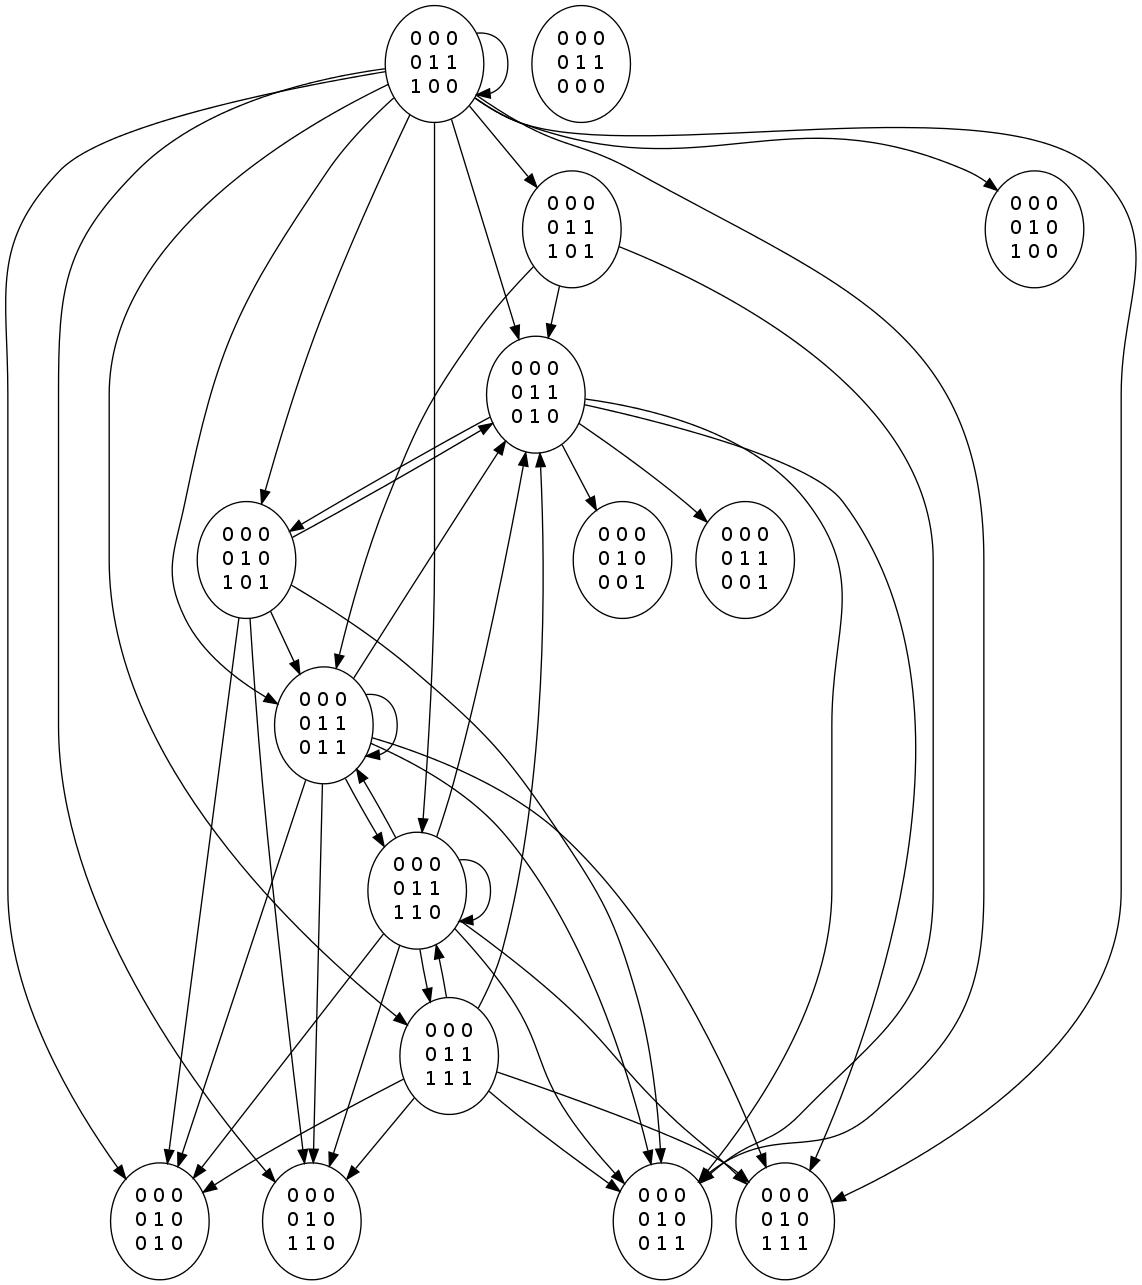
\includegraphics[scale=0.50]{graph_leftmost_mid.jpg}
\caption{Persistent cases}
\label{graph:leftmost_mid}
\end{figure}

\begin{figure}
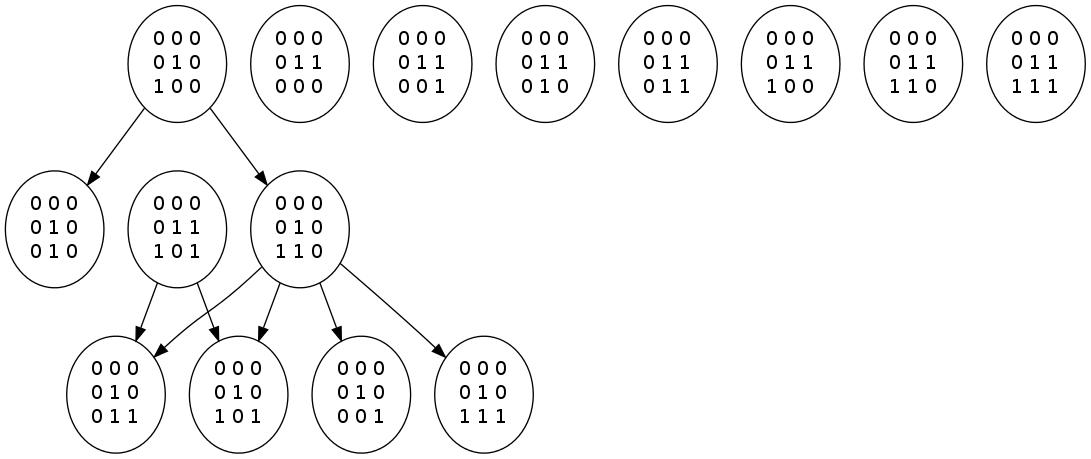
\includegraphics[scale=0.50, angle=90]{graph_leftmost_left.jpg}
\caption{"Go-left" cases}
\label{graph:leftmost_left}
\end{figure}

\end{document}
